%\documentclass[a4paper,10pt]{revtex4-1}
%\usepackage{tikz}

%\begin{document}

%\thispagestyle{empty}

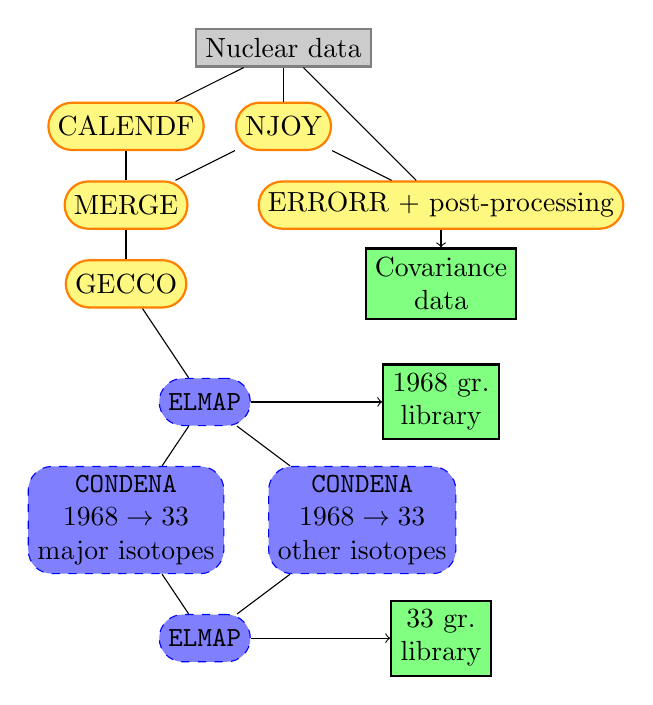
\begin{tikzpicture}[scale=1.0,
  data/.style={rectangle,draw=black!50,fill=black!20,thick},
  code/.style={rectangle,minimum size=6mm,rounded corners=3mm,fill=yellow!50,draw=orange,thick},
  lib/.style={rectangle,fill=green!50,draw=black,thick},
  emod/.style={rectangle,minimum size=6mm,rounded corners=3mm,fill=blue!50,draw=blue,dashed}]

  \pgfmathsetmacro{\ysep}{-1.0} ;
  
  \node[data] at ( 2, 0)       (nucdat)  {Nuclear data} ;
  \node[code] at ( 0, 1*\ysep) (calendf) {CALENDF} ;
  \node[code] at ( 2, 1*\ysep) (njoy1)   {NJOY}    ; 
  \node[code] at ( 0, 2*\ysep) (merge)   {MERGE}   ;
  \node[code] at ( 4, 2*\ysep) (errorr)  {ERRORR + post-processing}    ;
  \node[code] at ( 0, 3*\ysep) (gecco)   {GECCO}   ;
  \node[lib,align=center]  at ( 4, 3*\ysep) (cov)   {Covariance\\data} ;
  \node[emod] at ( 1, 4.5*\ysep) (elmap1)  {\texttt{ELMAP}}   ;
  \node[lib,align=center]  at ( 4, 4.5*\ysep) (lib1968)  {1968 gr.\\library}   ;
  \node[emod,align=center] at ( 0, 6*\ysep) (condena1)  {\texttt{CONDENA}\\$1968\rightarrow 33$\\major isotopes}   ;
  \node[emod,align=center] at ( 3, 6*\ysep) (condena2)  {\texttt{CONDENA}\\$1968\rightarrow 33$\\other isotopes}   ;
  \node[emod] at ( 1, 7.5*\ysep) (elmap2)  {\texttt{ELMAP}}   ;
  \node[lib,align=center]  at ( 4, 7.5*\ysep) (lib33)  {33 gr.\\library}   ;

  \draw[]   (nucdat)   -- (calendf) ;
  \draw[]   (nucdat)   -- (njoy1) ;
  \draw[]   (nucdat)   -- (errorr) ;
  \draw[]   (njoy1)    -- (errorr) ;
  \draw[]   (njoy1)    -- (merge) ;
  \draw[->] (errorr)   -- (cov) ;
  \draw[]   (calendf)  -- (merge) ;
  \draw[]   (merge)    -- (gecco) ;
  \draw[]   (gecco)    -- (elmap1) ;
  \draw[->] (elmap1)   -- (lib1968) ;
  \draw[]   (elmap1)   -- (condena1) ;
  \draw[]   (elmap1)   -- (condena2) ;
  \draw[]   (condena1) -- (elmap2) ;
  \draw[]   (condena2) -- (elmap2) ;
  \draw[->] (elmap2)   -- (lib33) ;

\end{tikzpicture}

%\end{document}

